\vspace{5em}
\section{Equipment and Method}

\subsection{Equipment}
\begin{itemize}
    \item 1 $\times$ LabQuest 2 and cables
    \item 1 $\times$ Vernier Motion Detector ($\pm \SI{1}{\milli\meter}$)
    \item 2 $\times$ Stiff springs
    \item 1 $\times$ Light spring
    \item 1 $\times$ Vernier Hanging Mass Set ($\SI{250}{\gram}/\SI{50}{\gram}$)
    \item 1 $\times$ Retort stand
    \item 1 $\times$ Bosshead clamp, spring hanger, and rod
    \item 1 $\times$ Scientific scale ($\pm \SI{0.01}{\gram}$)
    \item 1 $\times$ Computer with Logger Pro 3
\end{itemize}

\begin{figure}[h]
\centering
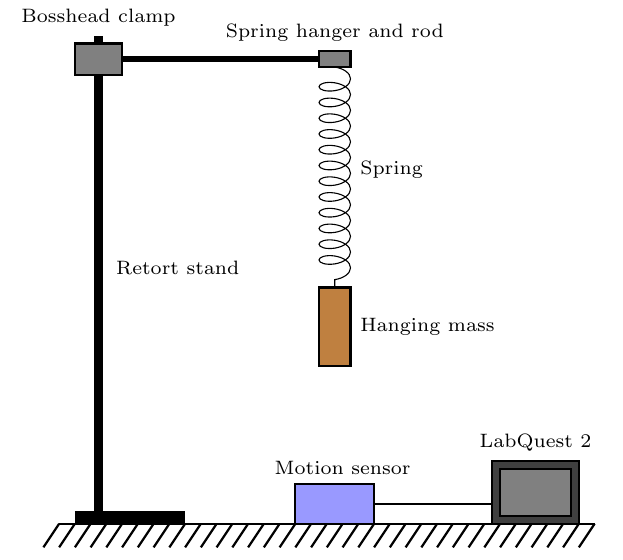
\begin{tikzpicture}[scale=1, every node/.style={font=\scriptsize}]
\useasboundingbox (-0.9,-0.6) rectangle (6.3,5.8);
% benchtop
\draw[thick] (-0.5,-0.5) -- (6.3,-0.5); % top surface
\foreach \x in {-0.5,-0.3,...,6.3} % diagonal hatch lines
    \draw[thick] (\x,-0.5) -- (\x-0.2,-0.8);

% retort stand
\draw[thick,line width=3pt] (0,-0.5) -- (0,5.7); % vertical rod
\draw[thick,line width=5pt] (-0.3,-0.42) -- (1.1,-0.42); % base

% horizontal rod
\draw[thick,line width=2pt] (0,5.4) -- (3,5.4); 

% bosshead clamp
\draw[thick, fill=gray] (-0.3,5.2) rectangle (0.3,5.6); 

% spring hook at end of rod
\draw[thick, fill=gray] (2.8,5.3) rectangle (3.2,5.5); 

% vertical spring
\draw[decorate,decoration={coil,aspect=0.5,segment length=2mm, amplitude=2mm}] (3,5.3) -- (3,2.5); 

% mass
\draw[thick, fill=brown] (2.8,2.5) rectangle (3.2,1.5); 

% wire to labquest
\draw[thick] (3.5, -0.25) -- (5, -0.25); 

% motion sensor
\draw[thick, fill=blue!40] (2.5,-0.5) rectangle (3.5,-0.0); 

% labquest
\draw[thick, fill=darkgray] (5,-0.5) rectangle (6.1,0.3);
\draw[thick, fill=gray] (5.1,-0.4) rectangle (6,0.2); 

% labels
\node[right] at (0.1,2.75) {Retort stand};
\node[above] at (0,5.7) {Bosshead clamp};
\node[above] at (3,5.5) {Spring hanger and rod};
\node[right] at (3.2,4) {Spring};
\node[right] at (3.2,2) {Hanging mass};
\node[above] at (3.1,0) {Motion sensor};
\node[above] at (5.55,0.3) {LabQuest 2};
\end{tikzpicture}
\caption{Experimental setup diagram for a vertical mass--spring system utilising a motion sensor.}
\end{figure}

\subsection{Method}
\begin{enumerate}
    \item Set up equipment as depicted in Fig.~2, with the light spring hooked onto the spring hanger and base of the retort stand towards the mass.
    \item Initialise the LabQuest 2 and Motion Detector and configure the mode to be displacement--time, sampling period to be $\SI{60}{\s}$, and sample rate to be $\SI{60}{\hertz}$.
    \item Connect the LabQuest 2 wirelessly to a computer with Logger Pro running.
    \item Measure and record the mass of the hanger from the Hanging Mass Set on a scientific scale.
    \item Attach the mass to the end of the spring and release it in a controlled manner, ensuring there is no horizontal displacement of the system before starting the data recording from the computer.
    \item Allow the $\SI{60}{\s}$ data collection period to finish without disturbing the system before removing the mass from the spring system.
    \item Apply a 'Damped Harmonic' curve fit in Logger Pro and record coefficients $A$, $B$, and $C$, and the $R^2$ value.
    \item Place a $\SI{50}{\gram}$ mass from the Hanging Mass set onto the hanger and measure and record the new total mass.
    \item Repeat steps 5 to 8 until at least 5 different masses have been trialled.
    \item Replace the light spring with a stiff spring and repeat steps 5 to 9.
    \item Replace the stiff spring with two stiff springs in series and repeat steps 5 to 9.
\end{enumerate}
